\section{Optical Character Recognition (OCR)}
Compilers are specifically design to understand these high-level programming languages and translate it to the machine code, but when it comes to read a document, it is difficult for them since document does not contains the rules similar to programming languages and in addition, every text documents have the basic blocks of any human language "letters". Character recognition techniques refers to a symbolic identity of a character within symbol or a character. This includes the replication/recognition of human functions like machine printed and hand printed/cursive-written characters by machines. Character recognition is known as optical character recognition since it deals with optically processed characters. The first mention of OCR was for as an aid to the visually handicapped and the first successful attempt was achieved by Russian Scientist Tyurin in 1900 \cite{govindan1990character}. Later on, the application of OCR changed into data processing systems in business world since it can deal with the enormous flood of paper documents such as bank cheques, commercial forms, credit card imprints, governmental records, mails and so on. Before smartphones and digital camera, documents were simply printed papers, However since smartphones and digital cameras got introduced, the number of documents increased since documents can now be easily produced digitally. Though generating documents got digitized, not all the documents are in machine readable or processable format. Most of them are just images or scans. Where OCR allowed to deal with these digitally born document such as scanned paper-documents, PDF files or images captured by a digital camera into machine readable, editable and searchable data. In paper \citep{AnOverviewoftheTesseractOCREngine} author have described in detail functionality of methods of famous Tesseract OCR Engine. Author talk about the development of open-source OCR engine "Tesseract" that it was develooped at HP between 1984 and 1994. In the infancy era for Tesseract, the accuracy was a challange, and it was major PhD reserch project in HP Labs Bristol. It was 1994, HP presented the final developed OCR engine to UNLV for the 1995 Annual Test of OCR Accuracy\cite{UNLV_4th_annual_test_ocr}, where it got prooved that it was worth against the commercial engines that exists that time. Later in 2005, HP made Tesseract for open source which is available at \url{http://code.google.com/p/tesseract-ocr}. According to \cite{AnOverviewoftheTesseractOCREngine}, the functionality of Tesseract OCR has been described in upcoming paragraphs.

\subsection{Line and Word Finding}
\subsubsection{Line Finding}

The line finding algorithm was developed to be able to work with images that are skewed without performing de-skew in order to maintain  the image quality \cite{Line_Finding_Algorithem}. The key role of this algorithm is to perform blob filtering and line construction. It uses a \textbf{simple percentile hight filter} for removing drop-caps and vertically touching characters, The \textbf{median height approximation} for text size and region and makes it safe to filter out blobs smaller than some fraction of the median height. By sorting x-coordinates, blobs are assigned to a unique text-lines. Later on, a least median of squares fir \cite{least_median_squares_algorithm} is being used for baseline estimation. Finally all blobs are being merged to form a line.

\subsubsection{Baseline Fitting}

After the line of the text document has been extracted, the baseline are fitted with more accuratly using a quadratic spline, an another first approch for OCR system that allowed Tesseract to handle curved baselines \cite{quadratic_spline_algorithm}. While quadratic spline have an advantage of claculating reasonably stable baseline, it can struggle when it comes to multiple spline segments. Therefore, the more traditional cubic spline \cite{Traditional_cubic_algorithm} has been used to perfom baseline fitting.

\begin{figure}[h]
    \centering
    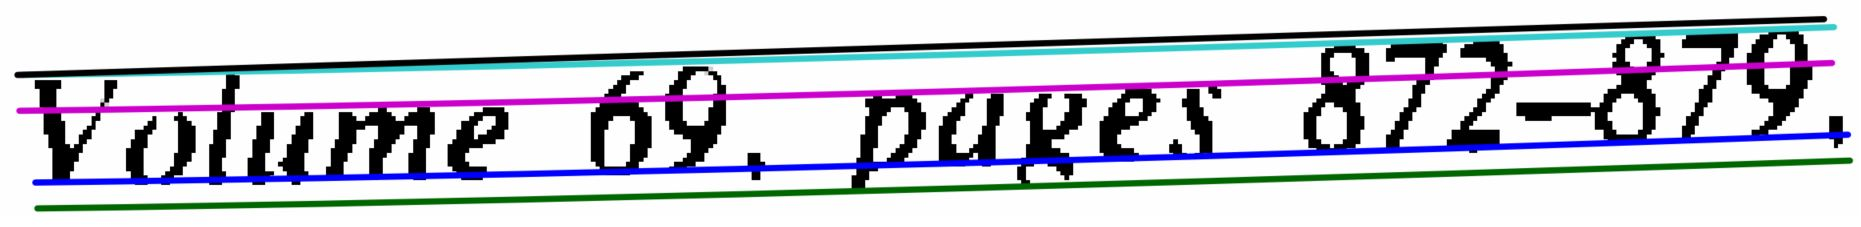
\includegraphics[width=0.7\textwidth]{chapters/images/OCR/Base_Line_Fitting.JPG}
    \caption{An example of a curved fitted baseline \cite{AnOverviewoftheTesseractOCREngine}}
    \label{fig:Baseline_Fitting}
\end{figure}

\Cref{fig:Baseline_Fitting} shows the fitted baseline, descender line, mean-line and ascender line. The black line is straight and cyan line is slightly curved with compare to the straight black line above it.

\subsubsection{Fixed Pitch Detection and Chopping}

Tesseract takes the text lines and finds the fixed pitch and chops the words into characters using the pitch. It also disables the chopper and associator on these words for word recognition. A typical example of chopping fixed-pitch word has been showed in \Cref{fig:Fixed_Pitch_detection}.

\begin{figure}[ht]
    \centering
    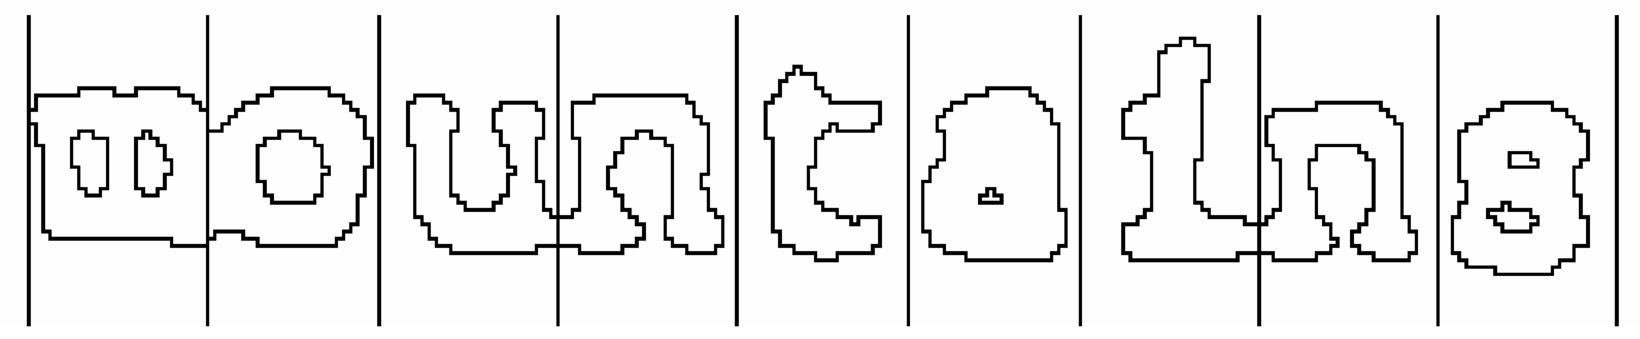
\includegraphics[width=0.7\textwidth]{chapters/images/OCR/Fixed_Pitch_detection.JPG}
    \caption{Fixed Pitch Detection and Chopping\cite{AnOverviewoftheTesseractOCREngine}}
    \label{fig:Fixed_Pitch_detection}
\end{figure}

\subsubsection{Proportional Word Finding}

\Cref{fig:Proportional_Word_Finding} shows a typical exmple of the problems when it comes to perform various task mention in previous paragraphs. For instance, (\RomanNumeralLows{1}) The units of '11.9\%' is clearly larger than the kerned of words 'erated'. (\RomanNumeralLows{2}) There is no horizontal gap at all between words 'of' and 'financial'.

\begin{figure}[ht]
    \centering
    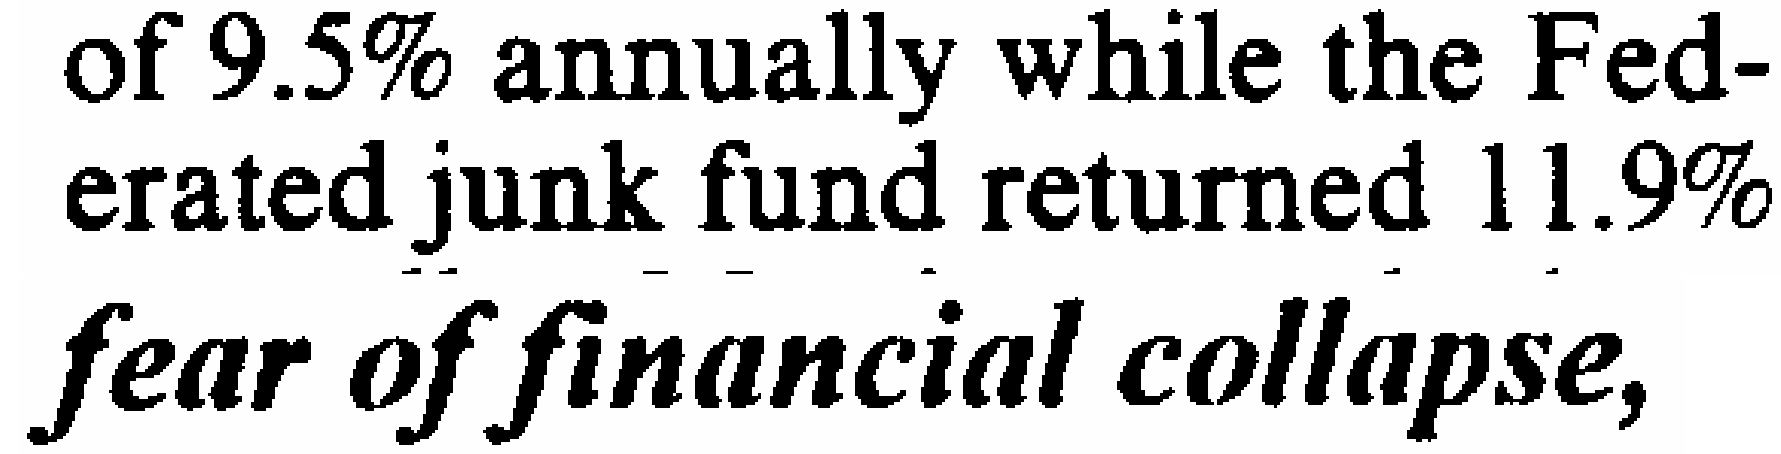
\includegraphics[width=0.6\textwidth]{chapters/images/OCR/Word_Finding.JPG}
    \caption{Proportional Word Finding\cite{AnOverviewoftheTesseractOCREngine}}
    \label{fig:Proportional_Word_Finding}
\end{figure}

Tesseract uses measurements of gaps in limited vertical range between the baseline and mean line. The spaces with smallest threshold are made fuzzy which later will be classified in word recognition.



\subsection{Overview of post process after Line and Word Finding}

Once the lines and words from the documents have been found, the step "Word Recognition" \cite{AnOverviewoftheTesseractOCREngine} is performed to identify the word segmentation which will be letter on classified. Tesseract performs "Chopping Joined Characters" in order to improve the results by chopping the blob based on the confidence derived from classifier. After the elimination of non potential chops, if the word is still not good enough, an associator makes an A* (best first) search based on  segmentation graph of possible combinations. This step can help Tesseract to identify the broken characters with more accuracy. Later on a "Static Character Classifier" \cite{AnOverviewoftheTesseractOCREngine} generates the 3-dimensional, (x, y, position, angle) with 50-100 features and the prototype features are 4-dimensional (x, y, position, angle, length) in a character. Which than will be used to perform classification to assign classes. The results of the Tesseract OCR is then exported to text, word or HTML format.